% ********** Chapter 1 **********

\section{Implementierung}
\label{sec:chap1:impl}

Im Folgenden wird beschrieben wie die in den beiden vorherigen Kapiteln \ref{sec:chap1:ana} und \ref{sec:chap1:design}
gewonnenen Erkenntnisse umgesetzt wurden. Jede in \ref{sec:chap1:ana:ap} gefundene Anforderung wird - soweit sinnvoll
m"oglich - in einem eigenen Unterkapitel aufgef"uhrt.

\subsection{Infrastruktur und ScriptEngine}
\label{sec:chap1:impl:1}

Um mit der Implementierung beginnen zu k"onnen musste zun"achst ein als dynamisch ladbare Bibliothek verf"ugbares
PHP erzeugt werden. Hierzu wurde von \cite{PHPHP} ein PHP in der Version 5.2.0 im Quelltext heruntergeladen und 
"ubersetzt, nachdem es mittels des Kommandozeilenparameters "'--enable-embed=shared"' konfiguriert wurde. Die so
erzeugte \emph{libphp5.so} konnte, zusammen mit den vorhandenen Headerdateien, zur Entwicklung genutzt werden.

Nun musste noch daf"ur gesorgt werden, dass sich die vom JSR 223 verlangten Klassen aus \ident{javax.script} im
Classpath befinden. Nachdem allerdings die Klassen aus der Referenzimplementation aus den zum Teil in 
\ref{sec:javanscripts:prototype} beschriebenen Gr"unden nicht in Frage kamen, wurde von \cite{JAVAHP} ein
\emph{Java Development Toolkit (JDK)} der Version 6 heruntergeladen. Da dieses JDK nicht als System-VM genutzt
werden kann wurde ein Makefile erstellt, welches die zur "Ubersetzung und Ausf"uhrung n"otigen Kommandos
vereinfacht.

Nachdem diese Vorarbeiten geleistet waren konnte mit der eigentlichen Implementierung begonnen werden.
Der erste Schritt war das Abbilden der ersten Anforderung (verf"ugbare ScriptEngines auflisten), erstens um 
sicherzustellen dass die Entwicklungsumgebung den Anforderungen gerecht wird, und zweitens um einen ersten
Eindruck der JSR 223 API zu erhalten. Also wurde im Package \texttt{samples} eine Klasse namens
\texttt{EngineList} geschrieben, die einen ScriptEngineManager erzeugt, und mittels der Methode
\texttt{getEngineFactories()} eine Liste aller verf"ugbaren ScriptEngines erstellt. Der Inhalt dieser
Liste wird dann mittels \texttt{System.out.println()} ausgegeben. 
Nachdem dem Makefile ein Target namens "'list"' hinzugef"ugt wurde, ergab ein erstes Ausf"uhren dieser Klasse
zum einen keine Fehler, und zweitens dass dem JDK 6 mit \emph{Mozilla Rhino} bereits eine ScriptEngine beiliegt:
\begin{lstlisting}[caption=erste Tests]
# make list
found 1 available ScriptEngines:
Engine: Mozilla Rhino
#
\end{lstlisting}

Im Folgenden wurde die Klasse \texttt{PHPScriptEngineFactory} erstellt, welche wie in Kapitel
\ref{sec:chap1:design:java} beschrieben
das Interface \texttt{ScriptEngineFactory} implementiert, hierbei erw"ahnenswert sind die Methoden 
\texttt{getProgram()} und \texttt{getMethodCallSyntax()}, erstere erstellt aus als Strings vorliegenden
einzelnen Anweisungen ein ausf"uhrbares PHP-Programm, zweitere erzeugt aus den "ubergebenen Parametern
einen der PHP-Syntax entsprechenden Methodenaufruf. Weiterhin enth"alt sie neben den weiter unten
beschriebenen nativen Methoden \texttt{startUp()} und \texttt{shutDown()} die Methode \texttt{read()}, die
aus einem "ubergebenen java.io.Reader eine Zeichenkette erstellt, die dann als Sourcecode verwendet
werden kann. Auf diese Weise kann der Anwender beispielsweise leicht seinen PHP-Quelltext in Dateien
verwalten, ohne jedesmal eigens einen Java-String erzeugen zu m"ussen.
Wurde nun die EngineList ausgef"uhrt stellte sich heraus, dass der ScriptEngineManager die neue ScriptEngine schon erkannte:
\begin{lstlisting}[caption=Neue ScriptEngine]
# make list
found 2 available ScriptEngines:
Engine: Mozilla Rhino
Engine: XP-Framework Turpitude PHP Engine
#
\end{lstlisting}

Nachdem dieser Schritt getan war, wurde mit der Erstellung der eigentlichen ScriptEngine begonnen. Deren
Implementierung gestalete sich sehr einfach, da durch das Ableiten der Klasse \texttt{AbstactScriptEngine} 
fast alle Varianten der \texttt{eval()}-Methode schon vorimplementiert waren, lediglich das Auslesen des
Skriptquelltextes aus einem "ubergebenen \texttt{Reader} musste selbst umgesetzt werden. 
Da\ss\ PHP urspr"unglich ausschlie\ss lich als CGI ausgef"uhrt wurde merkt man dem Kern der Sprache noch
deutlich an. So muss eine SAPI Funktionen aufrufen, welche den Beginn des sogenannten "'Requests"', respektive
dessen Ende anzeigen, auch m"ussen Funktionen zum setzen und lesen von HTTP-Headern und Cookies bereitgestellt
werden. Die n"otigen Aufrufe der Zend-Funktionen \texttt{php\_module\_startup()} und \texttt{php\_request\_startup}
werden in der PHPScriptEngine von zwei privaten, nativen Methoden erledigt: \texttt{startUp()} und \texttt{shutDown()}. 
Zus"atzlich wurde im Konstructor der PHPScriptEngine ein sogenannter "'ShutdownHook"' eingef"ugt, welcher daf"ur 
sorgt dass zumindest beim Herunterfahren der Virtual Machine shutDown() aufgerufen wird.

\subsection{"Ubersetzen und Ausf"uhren von Skripten}
\label{sec:chap1:impl:2}

Nachdem in Java die Grundlagen gelegt waren konnte mit dem Realisieren des nativen Teiles begonnen werden.
Die l"uckenhafte, an vielen Stellen sogar g"anzlich fehlende Dokumentation der Zend-Engine machte es unm"oglich
herauszufinden was der von den Zend-Entwicklern vorgesehene Weg ist, um PHP auf die beschriebene Art und Weise
einzubetten. Folglich musste durch reines Ausprobieren erraten werden wie vorgegangen werden sollte.
Zun"achst musste ein zur "Ubergabe an die Zend-Engine geeignetes \texttt{sapi\_module\_struct} definiert werden.
Hierbei handelt es sich um ein C-Struct, welches im Wesentlichen Pointer auf Callback-Funktionen enth"alt.
Viele dieser Funktionen, wie \texttt{read\_cookies} und \texttt{send\_headers}, wurden leer implementiert, da sie f"ur 
die geplante Art des Einsatzes nicht sinnvoll sind. Lediglich \texttt{error\_callback} soll hier erw"ahnt werden:
innerhalb dieser Methode werden zwei globale Variablen gesetzt, eine zeigt an ob die Fehlermethode aufgerufen wurde,
die andere h"alt die beim Aufruf ausgelesene Fehlermeldung vor, um sie sp"ater an den Benutzer weiterzugeben.
Ein erster Ansatz PHP-Code auszuf"uhren war die Zend-API Funktion \texttt{zend\_eval\_string}. Nachdem der n"otige
Boilerplate-Code geschrieben war zeigten sich auch Erfolge: eine in Java geschriebene HelloWorld-Klasse, welche
den Quelltext "'echo 'Hello World';"' direkt an die ScriptEngine weiterreicht, erzeugte die gew"unschte Ausgabe.
Eigehendere Tests unter Zuhilfenahme der \texttt{ScriptExec} Klasse, die ein Skript aus einer ihr "ubergebenen Datei
ausliest und an die ScriptEngine weitergibt f"orderten allerdings einen gravierenden Nachteil von zend\_eval\_string
zutage: Sobald als Parameter "'retval\_ptr"' nicht mehr \texttt{NULL} "ubergeben wird, wird nicht mehr das komplette
Skript, sondern nur noch die erste Zuweisung innerhalb des Quelltextes ausgef"uhrt. Wurde dieses Skript
\begin{lstlisting}[caption=Testscript f"ur zend\_eval\_string()]
$var = "Test";
for ($i=0; $i<10; $i++) {
    printf("Hello %s\n", $var);
}
\end{lstlisting}
mit retval\_ptr == NULL ausgef"uhrt, so wurde wie erwartet der Text "'Hello Test"' zehnfach auf der Konsole
ausgegeben. "Ubergab man allerdings einen Pointer auf ein valides zval-Struct so wurde nichts mehr ausgegeben,
und jener Struct enthielt als Wert den String "'Test"', und zus"atzlilch gab zend\_eval\_string einen Fehlercode
als eigenen R"uckgabewert zur"uck. Dieses Ph"anomen lies sich auch mit anderen, beliebig komplizierten Zuweisungen 
reproduzieren.

Obwohl der Versuch zend\_eval\_string zu nutzen fehlschlug konnten einige geschriebene Komponenten f"ur weitere
Ans"atze weiterverwandt werden, insbesondere die Funktionen \texttt{zval\_to\_jobject} zur Konvertierung des Zend-Engine
Datentypes \texttt{zval} in den JNI-Datentyp \texttt{jobject}, und \texttt{java\_throw}, die dass werfen von Java-Exceptions
aus dem nativen Teil heraus vereinfacht. 
Das Entwickeln der Funktion \texttt{zval\_to\_jobject} erwies sich aufgrund der fehlenden Dokumentation der Zend-Engine als
unerwartet kompliziert, insbesondere das Auslesen von Objekten aus zvals erfordert intimes Wissen "uber Zend-Engine Interna.
So werden beispielsweise Eigenschaften, \emph{Properties} genannt, analog zu den Elementen von Arrays intern 
in einer \texttt{Hashtable} gespeichert, wobei die Schl"ussel-Namen den Namen der Eigenschaft darstellen. Allerdings wird
dieser Schl"ussel im Falle von privaten und gesch"utzten (\texttt{protected}) Eigenschaften gesondert kodiert, in diesem
Falle beginnt er mit einem Nullbyte ($\backslash$0), gefolgt vom Namen der Objektklasse und einem weiteren Nullbyte und dem eigentlichen
Namen des Properties. Verst"andlicherweise sorgt diese Kodierung in C, wo das Nullbyte als Endzeichen f"ur Strings verwandt wird,
f"ur einige Probleme. "Uber die Beweggr"unde der Zend-Entwickler diese Kodierung w"ahlten kann nur spekuliert werden, aber 
die Vermutung liegt nahe, dass mit einem Nullbyte beginnende Strings in internen Funktionen, da sie f"ur C-Stringfunktionen die L"ange 0 haben,
als ung"ultig behandelt werden, und so einfach nirgendwo auftauchen. Da die Java-Klasse \texttt{PHPObject}, die laut Design an die JVM
zur"uckgegeben werden sollte wenn ein PHP-Objekt als R"uckgabewert auftaucht, allerdings alle
Attribute des jeweiligen PHP-Objektes enthalten sollte, mussten diese kodierten Attributnamen "'entwirrt"' werden.
Ein weiteres Problem das gel"ost wurde war, dass alle Zend-API Funktionen die
Quelltexte interpretieren erwarten, dass keine PHP-Tags mehr in diesem enthalten sind. PHP-Skripte werden "ublicherweise
innerhalb der Zeichenfolge "'$<$?php"' und "'?$>$"' eingeschlossen, um sie von den umgebenden Inhalten (meist HTML) abzugrenzen.
Die PHPScriptEngine filtert diese Zeichen automatisch aus dem Quelltextstrom.

Da zend\_eval\_string offensichtlich ungeeignet war die Anforderungen zu erf"ullen wurde nach einer Alternative gesucht, und
die Funktion \texttt{compile\_string} gefunden. Da diese - wie bereits der Name andeutet - den Quelltext lediglich in einen
\texttt{zend\_opcode\_array} "ubersetzt und dieser sp"ater ohnehin seperat ausgef"uhrt werden muss, wurde an dieser Stelle dem
geplanten Projektablauf vorgegriffen, und das Interface \texttt{Compilable} gleich mitimplementiert. Im Rahmen dieses Schrittes
wurde die Klasse \texttt{PHPCompiledScript} wie geplant realisiert. Diese enth"alt die native Methode \texttt{execute}, von welcher
der von der PHPScriptEngine erzeugte und in einen im PHPCompiledScript enhaltenen ByteBuffer geschriebene Opcode letztendlich
ausgef"uhrt wird. Hierzu sollte urspr"unglich die Zend-API Methode \texttt{execute()} verwandt werden, allerdings fuehrte jeglicher
Aufruf dieser Methode ausschliesslich zu Abst"urzen und Speicherfehlzugriffen, "uber deren Ursachen nur Vermutungen angestellt
werden k"onnen. Schlussendlich gelang es trotz aller Hindernisse Zend-Opcode fehlerfrei auszuf"uhren: die Zend-API Methode
\texttt{zend\_call\_function()} l"asst sich zur Ausf"uhrung jeglichen Opcodes missbrauchen, es ist lediglich notwendig einige
Typfelder des Opcode-Arrays mit "'falschen"' Informationen zu f"ullen. Zus"atzlich l"ost dieser Ansatz ein weiteres Problem:
Jede Funktion hat einen R"uckgabewert, aber im Gegensatz zu zend\_eval\_string wird dieser nicht direkt der Methode "ubergeben,
sondern in einem C-Struct des Types \texttt{zend\_fcall\_info} gespeichert und l"asst sich von dort erstens m"uhelos auslesen, und
weiterhin beeiflusst er das Ausf"uhrverhalten von zend\_call\_function nicht im Geringsten. Allerdings ergaben sich aus dieser 
Art und Weise Zend-Opcode auszuf"uhren auch einige Abweichungen zu einem "'Standard-PHP"':

Es war nicht mehr m"oglich Kommandozeilenparameter an das so ausgef"uhrte Script zu "ubergeben. Das ist vernachl"assigbar, da
JSR223 diese Art der Daten"ubergabe nicht vorsieht. Weiterhin erhielt der ansonsten innerhalb eines gew"ohnlichen Scriptes nutzlose
PHP-Befehl \texttt{return} pl"otzlich einen Sinn: das Script beendete sich und der R"uckgabewert wurde mit der zur"uckgegebenen
Variablen bef"ullt. Getreu dem Motto "'It's not a bug, it's a feature"' wurde dies allerdings nicht als st"orend empfunden, da
der normale \texttt{exit}-Befehl sich weiterhin wie gewohnt verhielt, und so nur zus"atzliche Funktionalit"at verf"ugbar wurde.

\subsection{Datenaustausch Java nach PHP}
\label{sec:chap1:impl:3}

Der n"achste Schritt war nun die "Ubergabe von Parametern aus Java an den PHP-Interpreter. Idealerweise sollten die zu "ubergebenen
Objekte nicht nur hin- und herkopiert werden, sondern sie sollten als Repr"asentation innerhalb der PHP-Umgebung verf"ugbar sein.
Dies bringt den Vorteil mit sich, dass nicht nur die Daten der Objekte, sondern auch deren Funktionalit"at dem PHP-Entwickler zur
Verf"ugung steht. Ausserdem sollte es dem Anwender m"oglich sein Java-Objekte aus PHP heraus zu erzeugen und Methoden auf diesen
Aufuzrufen.

Um dies zu erreichen war es n"otig Klassen "'von Aussen"', also ohne PHP-Quelltext zu nutzen, in den Interpreter zu injizieren,
und Aufrufe auf Objekte dieser Klassen auf C-Ebene abzuhandeln, da nur auf C-Ebene auf JNI-Funktionalit"at zugegriffen werden konnte. 
Diese Art von Klasse wird von Zend \emph{internal class} genannt, da sie nicht im PHP-Userspace, sondern direkt im Interpreter oder in von
ihm geladenen Bibliotheken implementiert werden.
Leider existiert auch zu dieser Seite der Zend-Engine keinerlei Dokumentation, und so musste viel ausprobiert werden um
herauszufinden wie dies zu bewerkstelligen w"are. Schliesslich wurde die Zend-Makro \texttt{INIT\_OVERLOADED\_CLASS\_ENTRY} entdeckt,
und nach vielen weiteren Versuchen wurde die Bedeutung des Makros und die restlichen Schritte herausgefunden, die n"otig
sind um eine solche interne Klasse zu erstellen:

Um der Zend-Engine eine Klasse unterzuschieben muss zun"achst ein C-Struct definiert werden das neben einem Struct von Typ
\texttt{zend\_object} namens \texttt{std} beliebige weitere Daten enthalten kann. Dieses Struct wird f"ur jede Instanz der Klasse
vorgehalten. Weiterhin wird ein Array vom Typ \texttt{function\_entry[]} ben"otigt, welches die Callbacks - im wesentlichen Funktionspointer
auf C-Funktionen - f"ur verschiedene Ereignisse auf dem Objekt enthalten. Im Gegensatz zu im Userland - in PHP also - implementierten
Methoden werden diese \emph{built-in functions} genannt.
Besonders erw"ahnenswert sind hier die Funktionen f"ur 
\texttt{\_\_call}, \texttt{\_\_get} und \texttt{\_\_set}, \texttt{\_\_call} wird bei jedem Methodenaufruf aufgerufen, und erh"alt neben dem
Funktionsnamen auch alle "ubergebenen Parameter, und bietet so die M"oglichkeit PHP-Methoden direkt in C zu implementieren, ohne f"ur jede
Methode einen eigenen Eintrag im Funktionspointerarray zu ben"otigen. Allerdings kann es bei solchen mittels \texttt{\_\_call} implementierter
Methoden zu "Uberschneidungen mit "'echten"' Methoden, solchen also die einen Eintrag im Funktionspointerarray haben, kommen. In solchen
F"allen wird immer zuerst "uberpr"uft ob im Array ein Eintrag passenden Namens existiert, und gegebenenalls diese Methode aufgerufen, bevor
der Aufruf an  \texttt{\_\_call} weitergereicht wird.
\texttt{\_\_get} und \texttt{\_\_set} werden bei jedem lesenden beziehungsweise schreibenden Zugriff auf ein nicht gefundenes Attribut des
Objektes aufgerufen, und erhalten neben dem neuen Wert auch den Namen des Attributes. Normale Attribute eines Objektes werden in einer
HashTable gespeichert und auch hier gilt: ist in der HashTable ein Attribut gesuchten Namens vorhanden wird dieses zur"uckgeliefert,
ansonsten wird je nachdem \texttt{\_\_get} oder \texttt{\_\_set} aufgerufen.

Weiterhin gibt es noch die beiden Funktionen
\texttt{\_\_construct} und \texttt{\_\_destruct}, die beim erzeugen beziehungsweise zerst"oren des Objektes aufgerufen werden,
die Funktionen \texttt{\_\_sleep} und \texttt{\_\_wakeup}, die beim serialisieren beziehungsweise deserialisieren des Objektes zum
Einsatz kommen, sowie die Funktion \texttt{\_\_cast}, die das Casten des Objektes auf einen anderen Datentyp implementieren soll.
Diese Funktionspointer werden zusammen mit dem Klassennamen an das Makro "ubergeben, um so einen sogenannten \texttt{zend\_class\_entry}
zu erzeugen, der f"ur jede Klasse ein mal global gespeichert wird.
Auf diese Art und Weise konnten die in 
\ref{sec:chap1:design:native} geforderten Klassen und deren Methoden implementiert werden. Alle Callback-Methoden haben keinen (\texttt{void})
als R"uckgabewert und m"ussen die Argumente entgegenehmen, die im Zend-API Makro \texttt{INTERNAL\_FUNCTION\_PARAMETERS} definiert werden.
Es enth"ahlt unter anderem einen Pointer auf den R"uckgabewert (\texttt{return\_value}), einen Pointer auf das Objekt (\texttt{this}), vor
allem aber ein Array der beim Aufruf der PHP-Methode "ubergebenen Argumente (\texttt{argv}) und einen Ganzzahlenwert, der die Anzahl
der Argumente enth"alt (\texttt{argc}).
Um allerdings "uberhaupt JNI-Funktionen nutzen zu k"onnen musste zun"achst die native Implementierung der startUp-Funktion der PHPScriptEngine 
erweitert werden: beim Aufruf dieser Funktion
wird der JNI-Evironment Pointer als globale Variable gespeichert, auch werden hier die Funktionen aufgerufen, die die Turpitude-Klassen
in die PHP-Umgebung injizieren.

\subsection{TurpitudeEnvironment}
\label{sec:chap1:impl:3}

Als erste wurde die Klasse \texttt{TurpitudeEnvironment} implementiert. Das Objekt-Struct enth"alt neben dem zend\_object noch pointer
auf den aktuellen ScripContext sowie die JNI-Umgebung. Eigene, f"ur PHP lesbare Attribute besitzt die Klasse nicht, also mussten
nur die geforderten Methoden umgesetzt werden. Zuvor wurde allerdings getestet, ob das injizieren der Klasse funktioniert hat, und die
ScriptEngine wurde derart angepasst, dass jedem Aufruf eines PHP-Skriptes eine Zeile vorangestellt wird, die eine Instanz der Klasse
erzeugt und in das PHP-Superglobal \texttt{\$\_SERVER} eingef"ugt wird. Superglobals sind eine Besonderheit von PHP, normale globale
Variablen m"uessen im Scope einer Funktion oder Methode mittels des Schl"usselwortes \texttt{global} bekannt gemacht werden, Superglobals
hingegen sind immer und von "uberall erreichbar. Der Name, unter dem das TurpitudeEnvironment dort eingef"ugt wird ist in der ScriptEngine
mittels der Methoden \texttt{setVarName()} und \texttt{getVarName()} konfigurierbar. Ein \texttt{var\_dump(\$\_SERVER)} zeigte, dass das
injizieren und initialisieren der Klasse funktioniert hatte.
\begin{lstlisting}[caption=TurpitudeEnvironment in \$\_SERVER einf"ugen]
$_SERVER["TURP_ENV"] = new TurpitudeEnvironment();
\end{lstlisting}
In allen Turpitude-Klassen wird hierzu in der Callback-Methoda \texttt{\_\_call} der 
Methodenname ausgelesen, der sich in \texttt{argv} and der Stelle [0] befindet. Ausserdem wird stets ein Pointer auf die zweite Stelle
von \texttt{argv}, sowie ein Integer der um eins kleiner ist als \texttt{argc}, an die die eigentlichen
Methoden implementierenden Funktionen "ubergeben, zusammen mit \texttt{return\_value} und eventuell dem dem Objekt-eigenen C-Struct.
Diese PHP-Methoden implementierenden Funktionen werden im weiteren Verlauf auch \emph{Handler} genannt.
Danach wird in jeder \texttt{\_\_call}-Funktion mittels \texttt{strcmp} der Name der aufgerufenen Methode mit den Namen der zu implementierenden 
Methoden verglichen, und falls eine "Ubereinstimmung gefunden wurde wird die jeweilige Funktion aufgerufen. Wird keine "Ubereinstimmung
gefunden wird mittels des Makros \texttt{php\_error} ein PHP-Laufzeitfehler erzeugt. Da diese Fehler von Turpitude von der Funktion
\texttt{turpitude\_error\_cb} als \texttt{PHPEvalException} an die JVM weitergeleitet werden stellen sie ein probates Mittel zum Abbruch
der PHP-Programmausf"uhrung dar, und k"onnen gefahrlos eingesetzt werden. 
Diese Gefahrlosigkeit r"uhrt daher, dass Turpitude alle Aufrufe von Zend-Funktionen durch einen speziellen Try-Catch Block einschliesst:
\begin{lstlisting}[caption=Zend Try-Catch Block]
zend_first_try {
    // Aufrufe
} zend_catch {
    // Fehlerbehandlung
} zend_end_try();
\end{lstlisting}
Ohne diese Zeilen w"urden schwerwiegende PHP-Fehler einen sofortigen Abbruch des laufenden Prozesses durch den C-Systemaufruf
\texttt{\_exit} mit dem Fehlercode 255 zur Folge haben, was in diesem Falle nicht nur den PHP-Interpreter, sondern auch die gesamte 
einbettende Java Virtual Machine beenden w"urde. Im Catch-Block findet die Fehlerbehandlung statt, im Normalfall wird hier eine
Java-Exception, mit dem Text der PHP-Fehlermeldung, geworfen und der Interpreter beendet. Leider f"uhren auch einige PHP-Funktionen
(genauer: alle Funktionen die die Zend-Funktion \texttt{zend\_bailout} aufrufen)
zu einem Sprung in den Catch-Block, weswegen in der oben beschriebenen Funktion \texttt{turpitude\_error\_cb} eine globale Variable
gesetzt werden muss, die anzeigt, ob ein echter Fehler aufgetreten ist.

\subsection{Java-Klassen in PHP}
\label{sec:chap1:impl:4}

Die erste Methode des TurpitudeEnvironment, die implementiert wurde war \texttt{findClass()}. In der zugeh"origen C-Funktion wird zun"achst 
lediglich "uberpr"uft, ob die Anzahl der Parameter stimmt, und ob der "ubergebene Parameter vom Typ \texttt{String} ist. Dann wird die
zur Klasse \texttt{TurpitudeJavaClass} geh"orende Funktion \texttt{make\_turpitude\_jclass\_instance} aufgerufen, die eine TurpitudeJavaClass
zur"uckgibt. Um eine Instanz dieser
Klasse erzeugen zu k"onnen musste diese allerdings zun"achst dem Interpreter bekannt gemacht werden, dies geschah analog zum Bekanntmachen
von TurpitudeEnvironment. Die Funktion \texttt{make\_turpitude\_jclass\_instance} selbst erwartet drei Argumente, eine \texttt{jclass} der zu
repr"asentierenden Klasse, deren Klassennamen und einen Pointer auf den zval, der das Objekt enthalten soll. Da die TurpitudeJavaClass 
tats"achlich Attribute (den Klassennamen) enthalten soll, muss die Zend-HashTable initialisiert werden, die diese Attribute enthalten soll.
Dies geschieht mittels der Zend-Funktion \texttt{object\_init\_ex}, die neben einem zval-Pointer den class\_entry entgegennimmt.
Nachdem im entsprechenden \texttt{object\_struct} die jclass gesetzt wurde konnte schlussendlich "uber die Funktion \texttt{zend\_hash\_update} 
der Klassenname in die HashTable eingef"ugt werden. Ein var\_dump einer solchen Klasse sah nun wie folgt aus:
\begin{lstlisting}[caption=Dump einer TurpitudeJavaClass]
object(TurpitudeJavaClass)#4 (1) {
  ["ClassName"]=>
    string(16) "java/lang/String"
}
\end{lstlisting}
Um aus Klassen Objekte erzeugen zu k"onnen muss ein Konstruktor aufgerufen werden. Konstruktoren werden im JNI wie ganz normale Methoden
behandelt, nur dass der Methodenname stets \texttt{$<$init$>$} ist. Um mittels JNI eine Methode aufrufen zu k"onnen muss diese zuerst in
Form einer Variablen des Types \texttt{jmethodID} vorhanden sein, die wiederum mit der JNI-Umgebung und einer \texttt{jclass} erzeugt werden kann.
Hierzu muss neben dem Methodennamen allerdings auch die Signatur der aufzufindenden Methode angegeben werden, und zwar in einer speziellen
Syntax. Diese zu erl"autern w"urde an dieser Stelle den Rahmen sprengen, deswegen hier nur der Verweis auf die JNI-Dokumentation, zu finden
unter \cite{JNIHP}.
Um eine jmethodID f"ur den PHP-Anwender hantierbar zu machen wurde die Klasse TurpitudeJavaMethod eingef"uhrt, wieder analog zu den
vorherigen Klassen. Eine TurpitudeJavaMethod hat weder Attribute noch eigene Methoden, sie wird ausschliesslich als Parameter in Methoden
anderer Klassen ben"otigt. Erzeugt wird ein solches Objekt mit der Methode \texttt{findMethod()} der Klasse TurpitudeJavaClass, die zwei 
String-Argumente erwartet: den Methodennamen und die JNI-kodierte Methodensignatur. Die Validit"at dieser beiden Argumente wird nicht explizit
gepr"uft, wird keine entsprechende Methode gefunden wird ein PHP-Fehler erzeugt. Die TurpitudeJavaClass wird durch die Funktion
\texttt{make\_turpitude\_jmethod\_instance} erzeugt, und speichert neben ihrem Namen und ihrer Signatur noch einen Indikator der anzeigt
ob sie statisch aufgerufen werden kann. Ausserdem wird im object\_struct die jclass und der im enum \texttt{turpitude\_java\_type} definierte
Typ des R"uckgabewertes gespeichert. Dieser wird durch parsen der Signatur ermittelt und wird sp"ater beim Aufruf der Methode ben"otigt.
Neben den einfachen Java-Datentypen wie \texttt{int}, \texttt{boolean} und \texttt{double} werden noch \texttt{void} und vor allem \texttt{Object} unterschieden,
wobei der eigentliche Typ des Objektes keine Rolle spielt.
Neben der Methode \texttt{findMethod()} wurde in der TurpitudeJavaClass noch die Methoden \texttt{findStaticMethod()} f"ur statisch
aufrufbare Methoden und \texttt{findConstructor()}, die dem Anwender die "Ubergabe von "'$<$init$>$"' als Methodenname erspart, definiert.

\subsection{Java-Objekte in PHP}
\label{sec:chap1:impl:5}

Derart erstellte Konstruktoren konnten nun zur Erzeugung von Java-Objekten genutzt werden. Diese sollten in PHP durch die Klasse
\texttt{TurpitudeJavaObject} dargestellt werden, und so musste diese zun"achst dem Interpreter auf be"ahrte Weise bekanntgemacht werden.
Neben dem \texttt{jobject}, welches das Java-Objekt auf C-Ebene repr"asentiert wird im object\_struct des TurpitudeJavaObject noch die \texttt{jclass}
mitgespeichert, was sp"ater klassenspezifische Operationen erleichtern soll. Das Objekt selbst wird schon im call-Handler der TurpitudeJavaClass 
erzeugt, und zwar mittels der JNI-Funktion \texttt{NewObject}, falls der Konstruktor keine Argumente erfordert, und er Funktion \texttt{NewObjectA} falls
er Argumente erwartet. Alle JNI-Funktionen mit dem Suffix "'A"' am Ende erwarten die an die Java-Methode weiterzureichenden Argumente als Array
des Types \texttt{jvalue}, einem Union aller JNI-Typen. Um ein solches Array f"ullen zu k"onnen wurde die Funktion \texttt{zval\_to\_jvalue} geschrieben,
die "uber den Typen des zval ermittelt welches Attribut des jvalue bef"ullt werden soll. Leider enth"alt ein jvalue keinerlei Typinformation "uber den
gespeicherten Wert, was sp"ater bei der R"uckumwandlung eines jvalue in einen zval zu Problemen f"uhren k"onnte. Im Gegensatz zur oben beschriebenen 
Funktion \texttt{zval\_to\_jobject} wandelt \texttt{zval\_to\_jvalue} scalare PHP-Typen nicht in deren Objekt"aquivalente in Java, sondern in die
entsprechenden simplen Java-Typen um. Somit k"onnen auch Konstruktoren (und sp"ater auch Methoden) aufgerufen werden die solche Typen als Argumente
verlangen, ohne sich auf das Autoboxing der JVM verlassen zu m"ussen.
Um aus einem jobject eine Instanz der Klasse
TurpitudeJavaObject zu konstruieren wird es, zusammen mit der zugeh"origen Klasse - sowohl die jclass als auch die TurpitudeJavaClass - an die Funktion 
\texttt{make\_turpitude\_jobject\_instance} "ubergeben, in der die eigentliche Instanz angelegt und die Turpitude-Klasse als Attribut "'Class"' hinzugef"ugt wird. 
Eine so erzeugte Repr"asentation eines Java-Objektes vom Typ java.util.Date sieht f"ur den PHP-Anwender wie folgt aus:
\begin{lstlisting}[caption=Dump eines TurpitudeJavaObject]
object(TurpitudeJavaObject)#6 (1) {
  ["Class"]=>
  object(TurpitudeJavaClass)#4 (1) {
    ["ClassName"]=>
    string(14) "java/util/Date"
  }
}
\end{lstlisting}

\subsection{Java-Methodenaufrufe in PHP}
\label{sec:chap1:impl:6}

Nun konnte endlich der Aufruf von Java-Methoden implementiert werden. Der call-Handler des TurpitudeJavaObjects "uberpr"uft zuerst, ob es sich bei der
aufgerufenen Methode um \texttt{javaInvoke} handelt. Ist dies der Fall wird die Methode des Java-Objektes aufgerufen, die im ersten Parameter "ubergeben 
wurde. Danach wird - "ahnlich wie bei Konstruktoren - unterschieden, ob neben der aufzurufenden Methode noch andere Argumente "ubergeben wurden, in diesem
Fall wird - wieder wie bei Konstruktoren - ein Array aus jvalues erstellt und je nach Typ des R"uckgabewertes der Methode die entsprechende JNI-Funktion
(Call$<$type$>$MethodA) aufgerufen. Wurden ausser der Methode keine weiteren Parameter mit"ubergeben, wird eine entsprechende Funktion der Signatur
Call$<$type$>$Method (ohne A) aufgerufen. Der R"uckgabewert der aufgerufenen JNI-Funktion wird in einem jvalue gespeichert, der zusammen mit dem
Typen des R"uckgabewertes der Funktion \texttt{jvalue\_to\_zval} "ubergeben wird, die letztendlich den zval erzeugt, der an PHP zur"uckgegeben wird.
Im Zuge der Implementierung von Methodenaufrufen bei Objekten wurde auch gleich der Aufruf statischer Methoden bei Klassen implementiert, dieser funktioniert exakt 
gleich, nur dass JNI-Funktionen der Signatur CallStatic$<$Type$>$Method(A) aufgerufen werden m"ussen. Zu diesem Zweck wurde die TurpitudeJavaClass um die Methode
\texttt{invokeStatic} erweitert.

Da das erzeugen m"ussen von Methoden bevor man sie aufrufen kann doch eher m"uhsam erscheint wurde call-Handler noch derart erweitert, dass wenn keine der
explizit definierten Methoden aufgerufen wurde nicht einfach ein Fehler erzeugt wird, sondern es wird versucht eine Methode gleichen Namens zu finden und diese
aufzurufen. Dazu muss der Anwender allerdings als erstes Argument die Methodensignatur angeben, da es das JNI leider erm"oglicht alle Methoden eines Namens
zu finden, um dann eventuell anhand der weiteren Argumente die richtige Methode zu finden. Ist der erste Parameter also ein String wird versucht eine
Methode zu finden die den Namen der in PHP aufgerufenen Methode tr"agt, und die den "ubergebenen String als Signatur hat. Ist dies der Fall wird einfach 
eine Instanz von TurpitudeJavaMethod erzeugt und an Stelle des Signaturstrings in das Argumentenarray geschrieben. Nun muss nur noch die Funktion aufgerufen
werden die auch die mittels \texttt{javaInvoke} aufgerufenen Methoden abhandelt. Folglich kann die Java-Methode \texttt{toString()} der Klasse \texttt{java.util.Date}
auf diese beiden Arten aufgerufen werden:
\begin{lstlisting}[caption=Zwei Arten die gleiche Methode aufzurufen]
$method = $class->findMethod('toString', '()Ljava/lang/String;');
$string = $date->javaInvoke($method);
oder
$string = $date->toString('()Ljava/lang/String;');
\end{lstlisting}

\subsection{Zugriff auf Java-Attribute in PHP}
\label{sec:chap1:impl:7}

Weiterhin sollte es dem Anwender erm"oglicht werden, auf Attribute eines Objektes zuzugreifen. F"ur Attribute m"ussen mit dem JNI - wie bei Klassen und Objekten auch -
Handler erzeugt werden, allerdings wurde hier auf eine eigene PHP-Klasse verzichtet, sondern es wurden einfach dem TurpitudeJavaObject zwei weitere Methoden hinzugef"ugt: 
\texttt{javaGet()} und \texttt{javaSet()}. \texttt{javaGet()} erwartet analog zu Methoden zwei Argumente, den Namen des Attributes und dessen Signatur, beides als Strings, 
letzteres wieder JNI-kodiert. Wie bei Methodensignaturen auch wird der Feldsignaturstring geparst, um sp"ater dem R"uckgabewert den richtigen Typen zuweisen zu k"onnen, 
aber auch weil auch um ein Attribut eines Java-Objektes auszulesen die richtige JNI-Funktion aufgerufen werden muss. Diese Funktionen haben die Signatur
Get$<$Type$>$Field, und erwarten alle das Objekt dessen Attribut ausgelesen werden soll, sowie eine sogenannte \texttt{jfieldID}, die zuvor mittels der Funktion
\texttt{GetFieldID} generiert werden muss. Wie bei Methodenaufrufen der R"uckgabewert wird hier der Wert des Attributes in einem jvalue gespeichert, der wieder
in einen zval umgewandelt wird. \texttt{javaSet()} erwartet neben den Argumenten die auch \texttt{javaGet()} erwartet noch den Wert auf den das Attribut gesetzt werden
soll, daf"ur gibt diese Methode nat"urlich keinen Wert zur"uck. Auch \texttt{javaSet()} entscheidet anhand der Signatur welche JNI-Funktion zum Setzen des
Attributes aufgerufen werden soll, welche die Signatur Set$<$Type$>$Field haben, und versucht ebenfalls anhand des "ubergebenen Attributnamens und -Signatur die
entsprechende jfieldID zu finden.

Analog zu Feldern von Instanzen sollte auch auf statische Felder in Java-Klassen zugegriffen werden k"onnen, hierzu wurden in der TurpitudeJavaClass zwei Methoden
implementiert, \texttt{getStatic()} und \texttt{setStatic()}. Wie bei nicht-statischen Attributen auch m"ussen zum Setzen beziehungsweise Auslesen je nach Feld-Typ spezielle 
JNI-Funktionen aufgerufen werden, diese haben die Signatur Get/SetStatic$<$Type$>$Field. Die Umwandlung des zu setzenden Wertes beziehungsweise des R"uckgabewertes
geschieht analog zu nicht-statischen Attributen.

\subsection{Java-Exceptions in PHP}
\label{sec:chap1:impl:8}

Nachdem man nun Klassen konstruieren, deren Methoden aufrufen und auf deren Attribute zugreiffen konnte wurden die M"oglichkeiten der Fehlerbehandlung
verbessert. Java arbeitet haupts"achlich mit Exceptions, und auch die Turpitude-intern erzeugten Fehler treten in der JVM als Exceptions auf. Folglich mussten dem
Anwender Werkzeuge zur Hand gegeben werden, geworfene Exceptions in PHP zu fangen und zu behandeln, und selbst Java-Exceptions zu erzeugen. Das Werfen von
Exceptions kann der Anwender mittels der Methoden \texttt{throw} und \texttt{throwNew} des TurpitudeEnvironment bewerkstelligen. Mit \texttt{throw} k"onnen Instanzen
der Klasse \texttt{java.lang.Throwable} geworfen werden, die der Anwender zuvor wie oben beschrieben erzeugt hat. \texttt{throwNew} hingegen erwartet zwei Parameter,
zum einen den Namen der zu werfenden Exception, zum anderen die Nachricht, die die Exception enthalten soll. Will der Anwender also komplizierte Exceptions mit
werfen, die zus"atzlich zur eigentlichen Nachricht noch zus"atzlich Information tragen soll wird er \texttt{throw} nutzen, f"ur den gro\ss teil der F"alle 
hingegen reicht \texttt{throwNew} v"ollig aus. Um Exceptions auch fangen zu k"onnen wurde die Methode \texttt{exceptionOccurred} eingef"uhrt, die die gleichnamige
JNI-Funktion aufruft, und die zuletzt geworfene und noch nicht gefangene Exception zur"uckgibt. Wird keine solche Exception gefunden wird NULL zur"uckgegeben,
derart gefundene Exceptions verbleiben allerdings in diesem Status. Um erfolgreich behandelte Exceptions aus diesem Zustand zu entfernen wurde die Methode
\texttt{exceptionClear} implementiert, die ebenfalls keine Parameter entgegennimmt, und ebenfalls die gleichnamige JNI-Funktion aufruft.

Alle hier beschriebenen Methoden erzeugen PHP-Laufzeitfehler sollte beispielsweise die Anzahl der "ubergebenen Argumente nicht stimmen, oder falschen Types sein.
Wichtig ist noch zu bemerken, dass sowohl das Aufrufen von Java-Methoden, als auch das lesen beziehungsweise schreiben von Attributen auch auf nicht-"offentlichen
Methoden und Attributen funktioniert, einerseits da JNI keinerlei M"oglichkeiten bietet Zugriffsmodifikatoren zu erkennen, andererseits da man eigentlich davon
ausgehen k"onnen sollte, dass ein Anwender wenigstens in groben Z"ugen weiss was er tut. 

\subsection{Der JSR223 ScriptContext}
\label{sec:chap1:impl:9}

Mit der geleisteten Vorarbeit war es nun einfach die Anforderungen des JSR nach einem ScripContext umzusetzen. Die von der PHPScriptEngine erweiterte Klasse
AbstactScriptEngine bringt eine Kontextimplementation namens SimpleContext mit. Dieser Kontext wird beim Aufruf der nativen Methode \texttt{exec} des PHPCompiledScripts
als jobject "ubergeben und global gespeichert. An diesen Kontext kommt der Anwender in PHP "uber die Methode \texttt{getScriptContext} des TurpitudeEnvironment. Im 
entsprechenden Handler wird die Klasse des ScripContext ermittelt, damit eine TurpitudeJavaClass erstellt, und mit dem Kontext-jobject zu einer Instanz von
TurpitudeJavaObject vereinigt. Somit kann der Anwender einfach die entsprechenden Java-Methoden dieses Objektes aufrufen, um an die im Kontext enthaltenen Daten zu
gelangen. Getestet wurde das mit einem Programm das einen java.util.StringBuffer erzeugt, in den Kontext einsetzt, und dann ein PHP-Skript ausf"uhrt, das diesem
StringBuffer einen Text anh"angt. Nachdem das Skript ausgef"uhrt wurde enth"alt der StringBuffer sowohl die per Java, als auch die in PHP angeh"angten Zeichen.

\subsection{Implementieren des Interface Invocable}
\label{sec:chap1:impl:10}

Bis zu diesem Zeitpunkt konnte die Java-Applikation, die das PHP-Skript einbettet, dieses nur ausf"uhren, es konnten keine gezielten Aufrufe von Funktionen und Methoden
abgesetzt werden, obwohl diese F"ahigkeit eine Bilbiothek wie Turpitude erst wirklich interessant macht. Deswegen wurde das JSR223-Interface \texttt{javax.script.Invocable}
implementiert, das genau an diesem Punkt ansetzt und Abhilfe schaffen soll. Leider zeigte sich auch hier dass die JSR223-Spezifikation an einigen Stellen
etwas undurchdacht wirkt: laut Spezifikation zollte die jeweilige ScriptEngine das Interface implementieren. Nun implementiert die PHPScriptEngine aber schon
das Interface \texttt{javax.script.Compilable}, es ist also nicht eindeutig auf welchem Skript die Aufrufe durchgef"uhrt werden sollen, und die Spezifikation schweigt
sich zu diesem Thema ebenfalls aus. Um dieses Problem zu l"osen wurde zun"achst das PHPCompiledScript derart abgewandelt, dass dieses \texttt{Invocable} implementiert,
weil der Kontext hier eindeutig ist. Der PHPScriptEngine wurde ein weiteres Attribut \texttt{lastScript} hinzugef"ugt, in welchem das zuletzt "ubersetzte 
PHP-Script gespeichert wird. Dieses Attribut wird bei jedem Aufruf der Methode \texttt{compile} gesetzt, womit sind auch ausgef"uhrte Skripte abgedeckt werden.
Die Invocable-Methoden der PHPScriptEngine leiten nun einfach alle Aufrufe an die entsprechenden Methoden des \texttt{lastScript} weiter.

\texttt{javax.script.Invocable} beinhaltet vier Methoden, von denen jeweils zwei sehr "ahnlich sind. Die Methode \texttt{invokeFunction} ruft sogenannte \texttt{top-level functions}
des Skriptes auf, also im globalen Scope definierte Funktionen. Da die in der nativen Methode \texttt{execute}, die wie oben beschrieben beim Ausf"uhren 
eines "ubersetzten Skriptes aufgerufen wird, benutzte Zend-API Funktion \texttt{zend\_call\_function} ein auszuf"uhrendes Op-Array erwartet, und da das Finden des
richtigen Abschnittes im Op-Array des PHPCompiledScripts sehr viel Aufwand bedeutet h"atte wurd ein anderer Weg gew"ahlt: die Funktion \texttt{call\_user\_function}, die
direkt eine im PHP-Skript vorhandene Funktion aufruft. Damit dies allerdings funktionieren kann muss zun"achst in den sogenannten \emph{Executor Globals}, erreichbar
"uber das Makro \texttt{EG}, das Feld \texttt{active\_op\_array}, welches das gerade Aktive Op-Array enthalten soll, auf das im PHPCompiledScript gespeicherte
Op-Array gesetzt werden.
Um den R"uckgabewert einer Funktion an die Java-Applikation weiterreichen zu k"onnen wurde noch ein zval initiert, und ein Pointer auf dessen Pointer wurde in den 
\emph{Executor Globals} an die Stelle \texttt{return\_value\_ptr\_ptr} geschrieben. Nach dem erfolgreichen Ausf"uhren der Funktion enth"alt dieser zval den R"uckgabewert,
und konnte folglich wie alle anderen R"uckgabewerte behandelt und an die JVM zur"uckgegeben werden.
Um die von Java aus als Array von Objekten "ubergebenen Funktionsargumente an die PHP-Funktion weiterleiten zu k"onnen wird Speicher f"ur ein Array
von zval-Pointern reserviert, und dieses Array wird mittels der Funktion \texttt{jobject\_to\_zval} gef"ullt. Das so erstellte Array wird schlussendlich der die PHP-Funktion
aufrufenden Zend-API Funktion \texttt{call\_user\_function} "ubergeben, zusammen mit einem den Funktionsnamen enthaltenden zval vom Typ String, der zu nutzenden 
Funktionstabelle und dem Pointer auf den R"uckgabewert. Gibt \texttt{call\_user\_function} nun ein \texttt{FAILURE} zur"uck ist ein Fehler aufgetreten, und es wird
eine Java-Exception geworfen, ansonsten hat das Aufrufen funktioniert.
Ganz "ahnlich wurde die Invocable-Methode \texttt{invokeMethod} implementiert, allerdings musste zun"achst das PHPObject noch um ein Feld erweitert werden, welches
eine Referenz auf den entsprechenden zval innerhalb des PHP-Interpreters h"alt. Hierzu wurde - ganz "ahnlich zum Speichern des Op-Arrays im PHPCompiledScript -
ein java.nio.ByteBuffer verwendet, in welchen einfach der zval-Pointer gespeichert wird. Beim Aufrufen einer Methode wird dieser Zeiger nun ausgelesen und
der Funktion \texttt{call\_user\_function} als zweiter Parameter "ubergeben. Da so stets die richtige Methode der richtigen Instanz aufgerufen wurde
beschreibt dieser Parameter offensichtlich das Objekt, auf dem die Funktion aufgerufen werden sollte. Anonsten verl"auft ein Methodenaufruf analog
zu einem Funktionsaufruf.

F"ur den Java-Entwickler stellt sich das Aufrufen von Funktionen und Methoden also wie folgt dar:
\begin{lstlisting}[caption=Aufrufen von PHP-Funktionen und -Methoden]
Invocable inv = (Invocable)engine.compile(/* PHP-Source */);
Object phpobj = inv.invokeFunction("foo", "function call");
Object retval = inv.invokeMethod(phpobj, "bar", "method call");
\end{lstlisting}
Zun"achst muss nat"urlich PHP-Quelltext zu einem PHPCompiledScript "ubersetzt, und dieses dann auf Invocable gecastet werden. Dann wird die PHP-Funktion "'foo"'
aufgerufen, und ihr ein String als einziges Argument "ubergeben. Diese Funktion gibt in diesem Fall ein PHPObject zur"uck, auf welchem in der letzten Zeile
die Methode "'bar"', wieder mit einem String als einzigem Argument, aufgerufen wird.

Unter Zuhilfename von \texttt{invokeMethod} konnten schliesslich die anderen beiden Methoden des Interfaces \texttt{Invocable} implementiert werden, die beide
den Namen \texttt{getInterface} tragen. Beiden Varianten dieser Methode wird eine Java-Klasse oder -Interface "ubergeben, und zur"uckgegeben werden muss eine 
Instanz dieser Klasse, deren Methoden in der Skriptsprache Implementiert sind. Der Unterschied zwischen beiden Methoden ist, dass einer von beiden 
zus"atzlich ein Objekt "ubergeben werden kann, welches als Implementierendes Objekt genutzt werden soll. Dies macht im Falle von Turpitude nur Sinn, wenn das 
"ubergebene Objekt ein PHPObject ist, von dem der Anwender weiss, dass es das geforderte Java-Interface implementiert. Letztere Methode wurde zuerst implementiert,
da hierzu schon alle Vorraussetzungen geschaffen waren, und keine einzige Zeile C-Code mehr geschrieben werden musste. Als erstes wird in der Methode gepr"uft, ob
das "ubergebene Objekt wirklich eine Instanz von PHPObject ist. Danach wird eine Instanz der Klasse \texttt{java.lang.reflect.Proxy} erzeugt, die innerhalb Javas
als ganz normale Instanz der "ubergebenen Klasse auftritt, intern aber alle Methodenaufrufe an einen sogenannten \texttt{InvocationHandler} weiterreicht.
Ein InvocationHandler ist ein Interface, welches in diesem Falle von der Klasse \texttt{PHPInvocationHandler} implementiert wird, die im Konstruktor
ein PHPCompiledScript, in dessen Kontext die Methodenaufrufe stattfinden sollen, und ein PHPObject auf dem die Methodenaufrufe durchgef"uhrt werden sollen erwartet.
Die eigentlichen Methodenaufrufe werden s"amtlich durch die oben beschriebene Methode \texttt{invokeMethod} des PHPCompiledScripts erledigt.
Die Implementierung der Variante von \texttt{getInterface} die kein Objekt mitbringt stellte allerdings ein Problem dar - wie sollte ein das Java-Interface implementierendes
PHP-Objekt gefunden werden? Auch hier schweigt sich die JSR223 Spezifikation leider aus, so wurde nach einigem "Uberlegen entschlossen einzig auf den Namen der Klasse zu
pr"ufen. So wurde dem PHPCompiledScript eine weitere native Methode namens \texttt{createInstance} hinzugef"ugt, die als einziges Argument den 
Klassennamen in Form eines Strings erwartet. Sie sollte versuchen eine PHP-Klasse des "ubergebenen Namens zu finden, und eine Instanz dieser Klasse neu zu erzeugen.
Da Invocable hierzu keine Parameter"ubergabe vorsah, konnten auf diese Weise nur PHP-Objekte erzeugt werden, die einen Konstruktor ohne Argumente besitzen, ist 
dies nicht der Fall wird ein Laufzeitfehler erzeugt. Zur Implementierung dieser Methode wurde die Zend-Funktion \texttt{zend\_lookup\_class} gefunden, die zu einem
Klassennamen einen \texttt{zend\_class\_entry} zur"uckgibt. Mit diesem Klasseneintrag kann mittels der schon vorher genutzten Funktion \texttt{object\_init\_ex}
eine Instanz der Klasse erzeugt werden, die dann an die JVM als PHPObject zur"uckgegeben wird. Wird auf diese Weise ein PHPObject gefunden, wird mit diesem
als zweitem Argument einfach die schon fertige Variante der Interfacemethode aufgerufen. Da PHP keine Punkte in Klassennamen erlaubt, und zumindest in
Version 5 keine Namespaces kennt, wurde beschlossen den sogenannten \emph{SimpleName}, den Namen wie er in der Quelltextdatei vorkommt also, der zu findenden Klasse 
zu benutzen. Abbildung \ref{fig:javaseq} soll den Ablauf eines solchen Aufrufes einer in PHP implementierten Methode darstellen. 

\begin{figure}[h]
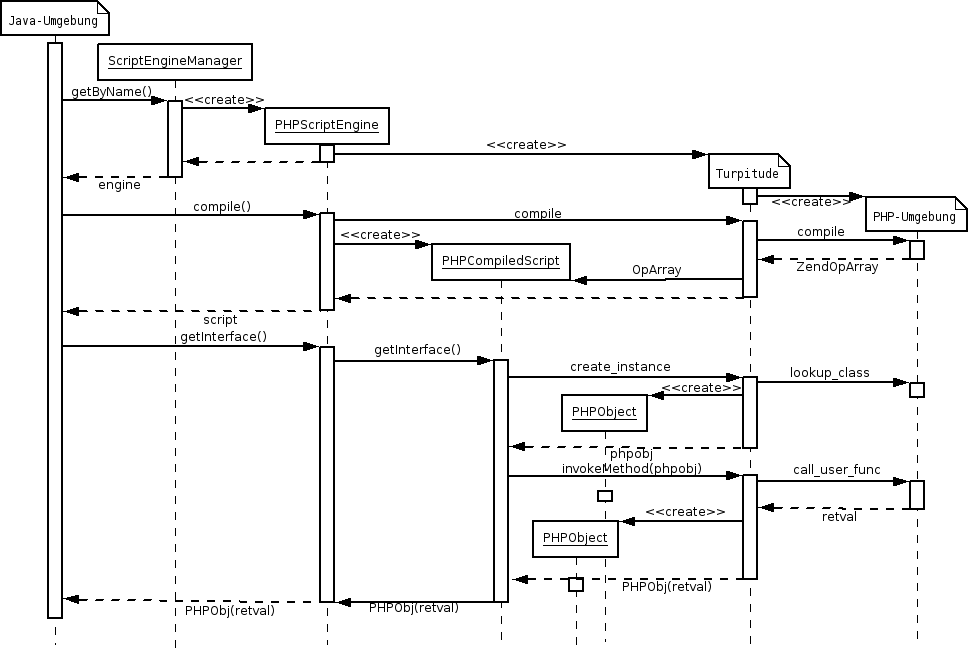
\includegraphics[width=\textwidth]{chap1/img/javaseq.png}
\caption{Ablauf eines in PHP implementierten Java-Methodenaufrufes}
\label{fig:javaseq}
\end{figure}

\subsection{Java-Arrays in PHP}
\label{sec:chap1:impl:11}

Eigentlich w"aren zu diesem Zeitpunkt alle Anforderungen an die Bibliothek erf"ullt, in vielen Bereichen sogar "ubererf"ullt gewesen, aber da w"ahrend
der Entwicklung festgestellt wurde, dass sowohl innerhalb als auch auch ausserhalb von 1\&1 erhebliches Interesse an Turpitude besteht wurde beschlossen 
einige Erweiterungen vorzunehmen, um Entwicklern ohne intimes Wissen "uber die Bibliothek das Entwickeln mit Turpitude zu vereinfachen.
Zum einen mussten einige Randbedingungen beim Aufrufen von Java-Methoden abgefangen werden, die sonst zu unerwarteten Ergebnisen f"uhren konnten, zum
anderen sollten Java-Arrays in PHP nicht nur als TurpitudeJavaObject dargestellt werden, sondern es sollte ein intuitiverer Umgang mit ihnen erm"oglicht werden.

Um Java-Arrays angemessen repr"asentieren zu k"onnen musste 
allerdings zun"achst eine neue Klasse eingef"uhrt werden, das \texttt{TurpitudeJavaArray}. Nach bew"ahrtem Muster wurden dieser Klasse drei Methoden
gegeben, zum einen \texttt{getLength}, die die L"ange des Arrays zur"uckgibt, und zum anderen \texttt{get} und \texttt{set}, um auf Elemente des Arrays zuzugreifen.
F"ur den Zugriff auf Java-Arrays bietet das Java Native Interface Funktionen an, die den Inhalt des Arrays in einen zusammenh"angenden Speicherbereich kopieren,
diese Funktionen haben die Signatur \texttt{Get$<$Type$>$ArrayElements}. Diese Speicherbereiche k"onnen  dann in C ausgelesen und ver"andert werden. 
Diese "Anderungen k"onnen beim Freigeben der Speicherbereiche entweder verworfen oder gespeichert werden. Da diese
Funktionen allerdings - wie fast alle JNI-Funktionen - f"ur jeden Typ andere sind, musste das oben beschriebene Parsen von JNI-Typstrings derart erweitert werden,
dass nicht nur Arrays sondern auch die verschiedenen Typen von Arrays erkannt werden. Das Freigeben der Speicherbereiche geschieht mittels der
Funktionen \texttt{Release$<$Type$>$ArrayElements}, deren letzter Parameter angibt ob die "Anderungen "ubernommen oder verworfen werden sollen.
Eine Ausname zu dieser Regel bilden Arrays von Objekten, auf deren Elemente direkt mittels der Funktionen \texttt{GetObjectArrayElement} und
\texttt{SetObjectArrayElement} zugegriffen werden kann.
Arrays in PHP sind eigentlich HashMaps, sie k"onnen also nicht nur numerische Werte, sondern jeglichen skalaren Typen als Index haben, folglich mussten
f"ur alle Zugriffe auf das \texttt{TurpitudeJavaArray} Tests eingebaut werden die nur numerische Indices zulassen.
Somit konnte zwar von PHP aus auf Java-Arrays zugegriffen werden,
allerdings eben nur mit den beschriebenen Methoden. Ein PHP-Anwender jedoch ist gewohnt mit dem Klammern-Operator [\texttt{index}] auf Arrays arbeiten zu k"onnen.
Damit auf eine Klasse in PHP wie auf ein Array zugegriffen werden kann bietet die Zend-Engine die M"oglichkeit das interne Interface \texttt{ArrayAccess} zu
implementieren, welches auf C-Ebene unter dem Symbol \texttt{zend\_ce\_arrayaccess} verf"ugbar ist. Dieses Interface enth"alt die Methoden \texttt{offsetGet} und
\texttt{offsetSet} um auf Arrays zuzugreifen, \texttt{offsetUnset} um Zeilen aus dem Array zu l"oschen und \texttt{offsetExists} um anzuzeigen ob zu einem
bestimmten Schl"usselwert ein Eintrag vorhanden ist. Die zu implementierenden Methoden wurden als \emph{built-in functions} in das bei der Initialisierung der
Klasse "ubergebene Funktionsarray eingetragen. Die Implementierung von \texttt{offsetUnset} erwies sich als trivial, da aus einem Java-Array keine
Zeilen gel"oscht werden k"onnen, es wird also lediglich ein PHP-Laufzeitfehler geworfen. Aufrufe von \texttt{offsetGet} und \texttt{offsetSet} werden lediglich
an die bereits implementierten Methoden \texttt{get} und \texttt{set} weitergereicht. 
\begin{lstlisting}[caption=Zugriff auf ein Java-Array]
$array = $instance->getStringArray('()[Ljava/lang/String;');
$length = $array->getLength();
$val = $array->get(0);
$array[0] = 'Wert';
\end{lstlisting}
Um dem PHP-Anwender den Umgang mit Java-Arrays weiter zu vereinfachen wurde beschlossen ein weiteres PHP-interne Interface zu implementieren, \texttt{IteratorAggregate}.
Dieses Interface beschreibt eine einzige Methode, \texttt{getIterator}, allerdings muss sie ein Objekt zur"uckgeben, das das PHP-Interface \texttt{Iterator} implementiert.
Ist dies der Fall kann der Anwender nicht nur mittels der \texttt{Iterator}-Methoden auf dem Array arbeiten, sondern auch mit dem \texttt{foreach}-Operator. Nachdem
das \texttt{TurpitudeJavaArray} so ver"aendert wurde dass es zus"atzlich das Interface \texttt{IteratorAggregate}, auf C-Ebene unter dem Symbol \texttt{zend\_ce\_aggregate}
zu finden, implementiert wurde also eine weitere Klasse eingef"uhrt, der \texttt{TurpitudeJavaArrayIterator}. Ein \texttt{Iterator} muss folgende Methoden implementieren:
\texttt{rewind}, \texttt{valid}, \texttt{key}, \texttt{current} und \texttt{next}, die alle keinerlei Argumente erwarten, und deren Funktionalit"at sich aus den Namen erschliessen 
sollte. Intern h"alt der \texttt{TurpitudeJavaArrayIterator} neben dem \texttt{TurpitudeJavaArray} "uber welces er iterieren soll noch einen Integer vor, der den
gerade aktuellen Index in das Array speichert. \texttt{rewind} setzt diesen Index auf 0 zur"uck, w"ahrend ein Aufruf von \texttt{next} ihn um eins erh"oht. \texttt{valid} gibt
genau dann \texttt{true} zur"uck wenn der Index gr"o\ss er als 0 und kleiner als die Anzahl der Elemente des Arrays ist. \texttt{key} gibt den aktuellen Index, \texttt{current}
das aktuelle Array-Element zur"uck, wozu einfach die \texttt{get}-Methode des entsprechenden Arrays aufgerufen wird. Hiernach konnte also in PHP folgenderma\ss en "uber Java-Arrays
iteriert werden:
\begin{lstlisting}[caption=Iterieren "uber ein Java-Array]
$iterator = $array->getIterator();
while ($iterator->valid()) {
    $row = $iterator->current();
    $ley = $iterator->key();
    printf("key: %d, val: %s\n", $key, $row);
    $iterator->next();
}
\end{lstlisting}
Laut Zend-Dokumentation sollte es eigentlich so sein, dass man "uber alle Objekte die entweder \texttt{Iterator} oder \texttt{IteratorAggregate} implementieren zus"atzlich mit
dem \texttt{foreach}-Operator itererieren k"onnen sollte. Dies stimmt wohl auch f"ur im Userland geschriebene Klassen, allerdings verursachte der Versuch auf diese Weise
"uber \texttt{TurpitudeJavaArray} oder \texttt{TurpitudeJavaArrayIterator} Objekte lediglich Abst"urze und Fehlermeldungen. Nach langem lesen von Zend-Quelltext
wurde entdeckt, dass jeder \texttt{zend\_class\_entry} ein Feld enth"alt, in dem ein Pointer auf eine Funktion gespeichert wird, die wiederum einen Pointer auf ein Struct vom Typ
\texttt{zend\_object\_iterator} zur"uckgeben muss. Solch ein Struct besteht im Wesentlichen aus einem Voidpointer (\texttt{void*}), in dem Daten gespeichert werden k"onnen, und
einem Pointer auf ein weiteres Struct, welches die Iteratorfunktionen enthalten muss. Folglich m"ussen interne Klassen nicht nur die Methoden implementieren mit denen der
Benutzer umgeht, sondern zus"atzlich noch Funktionen die die Zend-Engine benutzt um mit \texttt{foreach} "uber die Objekte zu iterieren. Nachdem sowohl die interne
\texttt{get\_iterator} Funktion als auch die internen Iteratorfunktionen, die fast eins-zu-eins Kopien der bereits implementierten Iteratormethoden sind - geschrieben waren
konnte nun auch mit dem \texttt{foreach}-Operator auf Java-Arrays zugegriffen werden:
\begin{lstlisting}[caption=Java-Array und foreach]
$iterator = $array->getIterator();
foreach ($iterator as $key => $val) {
    printf("key: %d, val: %s\n", $key, $row);
}
\end{lstlisting}

\subsection{Java-Methodenaufrufe, die 2.}
\label{sec:chap1:impl:12}

Eigentlich konnten zu diesem Zeitpunkt wie oben beschrieben schon Java-Methoden aus PHP heraus aufgerufen werden, allerdings hatte
diese Implementierung zwei Nachteile: einerseits musste der PHP-Entwickler die genaue JNI-Signatur der Methode kennen, andererseits -
und dies war der erheblich st"orendere Nachteil - konnten nur Methoden aufgerufen werden die tats"achlich in der Java-Klasse definiert
sind, auf der \texttt{findMethod()} aufgerufen wurde, also keine Methoden die in Oberklassen definiert wurden. Folglich musste der
PHP-Anwender unter Umst"anden mehrere Java-Klassen in PHP erstellen um unterschiedliche Methoden auf ein und demselben Java-Objekt
aufzurufen. Zwar mag es unter bestimmten Umst"anden w"unschenswert sein die genaue Methode angeben zu k"onnen die aufgerufen werden
soll, allerdings will man in den meisten F"allen doch von den Java-Sprechfeatures wie Polymorphismus profitieren. Aus diesem Grund
wurde beschlossen die Methodenaufrufe "uber \texttt{javaInvoke()} nicht zu ver"andern, aber die Methodenaufrufe "'direkt"' auf dem Objekt
so anzupassen, dass sie sich wie ein normaler Java-Methodenaufruf verhalten. Dies zu verwirklichen w"are mit JNI-Mitteln alleine
sehr schwer gewesen, weswegen auf die Java Reflection API zur"uckgegriffen werden musste.

Zu diesem Zweck wurde eine neue Java-Klasse erstellt, der \texttt{ReflectHelper}, die drei statische Methoden enth"alt:
\texttt{signatureMatchesArguments()}, \texttt{findMethod()} und \texttt{callMethod()}. 
\texttt{callMethod()} wird vom nativen Code aus aufgerufen, und erwartet als Parameter ein Objekt, einen Methodennamen und ein 
Array, welches Methodenargumente enth"alt, und versucht dann mit Hilfe der anderen beiden Methoden eine zum Namen und den Argumenten 
passende Methode auf dem "ubergebenen Java-Objekt zu finden und aufzurufen, und das Ergebnis dieses Aufrufes zur"uckzugeben.
Um die passende Methode zu finden nutzt sie \texttt{findMethod()}, welche aus der Klasse die verf"ugbaren Methoden ausliest, und 
zun"achst anhand des aufzurufenden Methodennamens, und schliesslich mit Hilfe von \texttt{signatureMatchesArguments()} anhand der
Argumententypen versucht die passende Methode zu finden. Eventuelle beim Aufruf auftretende Exceptions werden von \texttt{callMethod()}
einfach an den Aufrufer weitergeleitet, welcher diese Fehler dann selbst behandeln muss.

Nun musste der native Code des TurpitudeJavaObjects derart angepasst werden, dass jeder Methodenaufruf der nicht die explizit
definierten Methoden betrifft in einen Aufruf von \texttt{callMethod()} umgewandelt wird. Hierzu wurde eine C-Funktion geschrieben,
in der die zum Aufruf von \texttt{callMethod()} n"otigen jclass und jmethodID erzeugt, und die in PHP "ubergebenen Parameter
in ein Java-Array gewandelt werden. Ist dies geschehen wird \texttt{callMethod()} aufgerufen, und das Ergebnis wie bei jedem
anderen Java-Methodenaufruf auch in einen zval umgewandelt. Diese C-Funktion gibt "'true"' zur"uck wenn die Methode gefunden
und aufgerufen werden konnte, ansonsten wird "'false"' zur"uckgegeben. Dieser Bool'sche Wert wird dann im \texttt{\_\_call}-Callback
des TurpitudeJavaObjects ausgewertet, und es wird entweder das Ergebnis zur"uckgegeben, oder ein PHP-Laufzeitfehler erzeugt.
Der eigentliche Aufruf der Java-Methode geschieht "uber die Methode \texttt{invoke()} der gefundenen \texttt{Method}-Klasse, die neben
dem Objekt auf dem die Methode aufgerufen werden soll noch die zu "ubergebenden Argumente entgegennimmt.

Nun konnten Java-Methodenaufrufe in PHP auf die "Ubergabe der genauen Signatur verzichten, und es konnten auch Methoden aufgerufen
werden die in "ubergeordneten Klassen definiert wurden:
\begin{lstlisting}[caption=Verbesserter Aufruf einer Java-Methode]
$date = $obj->getDate();
$string = $date->toString();
\end{lstlisting}
Allerdings brachte diese Art des Methodenaufrufes auch Nachteile mit sich, die zum Teil mit der Reflection-API von Java,
und zum Teil mit Turpitude selbst zusammenh"angen. So werden beispielsweise Methodenargumente immer gem"a\ss  der Tabelle
\ref{tab:phptojava} konvertiert, was bei simplen Datentypen wie \texttt{int} und \texttt{float} unter Umst"anden zu Problemen f"uhren
kann, weil keine passende Methode gefunden wird. Beispielsweise f"uhrt folgender Code:
\begin{lstlisting}[caption=Typkonversionsfehler]
$date = $obj->setIntval(5);
\end{lstlisting}
zu einem Fehler, da der PHP-Wert (5) in einen java.lang.Long konvertiert wird, die Methode aber einen Integer erwartet.
Auch ist es so nur m"oglich "offentliche (\texttt{public}) Methoden aufzurufen,
bei privaten Methoden wirf \texttt{Method.invoke()} eine Exception.
In F"allen in denen der Anwender private oder ganz bestimmte Methoden aufrufen will l"a\ss t es sich also leider nicht vermeiden dass 
der Anwender auf \texttt{findMethod()} und \texttt{javaInvoke()} zur"uckgreiffen muss. In den allermeisten F"allen bringt diese "Anderung 
dem PHP-Programmierer aber eine erhebliche Vereinfachung, und rechtfertigt die entstehenden Nachteile, zumal ja in speziellen F"allen
auf die oben beschriebenen Methoden zur"uckgegriffen werden kann.

\subsection{Java-Attribute, die 2.}
\label{sec:chap1:impl:14}

Nachdem nun der Aufruf von Java-Methoden deutlich vereinfacht wurde, sollte eine "ahnliche Verbesserung beim Zugriff auf Java-Attribute
entwickelt werden, sprich der direkte Zugriff ohne den Aufruf einer speziellen Methode und vor allem ohne die Notwendigkeit die
Signatur des Attributes anzugeben. Weiter oben wurde beschrieben dass PHP-Klassen Callbacks f"ur das Setzen und Auslesen von 
Attributen besitzen, und diese sollten nun im TurpitudeJavaObject und in der TurpitudeJavaClass implementiert werden. Wie schon
im vorherigen Kapitel sollte hierzu die Java-Reflection API zur Hilfe genommen werden. Die Callbacks \texttt{\_\_get} und \texttt{\_\_set}
haben die selben Parameter die alle Methoden einer Zend-internen Klasse erwarten, und somit musste auch hier zun"achst der Feldname
und der Feld-Wert aus der Parameter-HashMap ausgelesen und zwischengespeichert werden. Der erste Parameter ist immer der Feldname,
und im Falle von \texttt{\_\_set} ist der zu setzende Wert an zweiter Stelle zu finden. Der Pointer auf den R"uckgabewert macht 
offensichtlich nur bei \texttt{\_\_get} Sinn, speichert aber in diesem Fall den ausgelesenen Wert. Beide Callbacks rufen statische Methoden
des in \ref{sec:chap1:impl:12} beschriebenen \texttt{ReflectHelper} auf, \texttt{getFieldValue()} und \texttt{setFieldValue()}, die beide
die Methode \texttt{getField()} der Klasse des Java-Objektes benutzen um das entsprechende \texttt{java.lang.reflect.Field} des Attributes 
zu finden, um dann auf diesem die Methode \texttt{get()} beziehungsweise \texttt{set()} aufzurufen. \texttt{getField()} geht nach folgendem
Algorithmus vor: Wenn die Klasse ein Feld mit dem gesuchten Namen definiert wird dieses zur"uckgegeben, ist dies nicht der Fall und die
Klasse implementiert mindestens ein Interface werden diese Interfaces nach einem passenden Feld durchsucht. Wird auch hier kein Feld
gefunden wird der Algorithmus rekursiv auf die Vaterklasse angewandt, hat die Klasse keine Vaterklasse wird ein Fehler erzeugt.
Die involvierten PHP-Variablen, beim
schreibenden Zugriff der zu schreibende Wert, beim lesenden Zugriff der ausgelesene Wert, werden wie immer nach den Tabellen
\ref{tab:phptojava} und \ref{tab:javatophp} konvertiert. Treten beim Zugriff Fehler auf, so wird die Ausf"uhrung des PHP-Codes abgebrochen
und ein entsprechender Fehler als Java-Exception geworfen. Nun konnte auf die Felder eines Java-Objektes wie folgt zugegriffen werden:
\begin{lstlisting}[caption=Verbesserter Zugriff auf Java-Attribute]
$obj->stringval = 'wert';
$str = $obj->stringval;
\end{lstlisting}
Im Zuge dieser Verbesserung wurde auch der direkte Zugriff auf statische Attribute von Java-Klassen erm"oglicht, indem die
Callbacks \texttt{\_\_get} und \texttt{\_\_set} in der TurpitudeJavaClass entsprechend implementiert wurden, sie unterscheiden sich
von den Callbacks des TurpitudeJavaObject lediglich darin, dass sie beim ReflectHelper die entsprechenden Methoden
\texttt{getStaticFieldValue()} und \texttt{setStaticFieldValue()} aufrufen.
Diese Methode des Zugriffs auf Java-Attribute hat die selben Nachteile wie der direkte Zugriff auf Java-Methoden, sprich es k"onnen
wieder nur "offentliche Felder gesetzt und ausgelesen werden, und die Typkonversion kann in manchen F"allen zu Problemen f"uhren, aber
auch hier "uberwiegen nach Meinung des Autors die Vorteile.

\subsection{Erzeugen von Java-Arrays in PHP}
\label{sec:chap1:impl:13}

In \ref{sec:chap1:impl:11} wurde beschrieben, dass Arrays die von Java an PHP "ubergeben werden als spezielles Objekt
mit speziellen Methoden abgebildet werden. Was allerdings noch fehlte war eine M"oglichkeit Java-Arrays in PHP zu erzeugen,
beispielsweise um sie als Argument an eine Methode zu "ubergeben. Das JNI bietet mit den Funktionen \texttt{New$<$Type$>$Array}
die M"oglichkeit beliebige Arrays zu erstellen, im Folgenden wird beschrieben wie diese Funktionen durch Turpitude in PHP
abgebildet und dem Anwender zug"anglich gemacht wurden.

Die Methode um neue Arrays zu erzeugen sollte \texttt{newArray()} hei\ss en, und da sie sich keiner Klasse zuordnen lie\ss  wurde 
sie dem TurpitudeEnvironment hinzugef"ugt. Sie erwartet zwei Argumente, zum einen den JNI-kodierten Typen der Arrayelemente 
als String, und zum anderen die L"ange, die das zu erzeugende Array haben soll. Intern wird das Erzeugen von der Funktion
\texttt{turpitude\_env\_method\_newarray()} "ubernommen, die die selben Parameter entgegennimmt wie die meisten PHP-Methoden
implementierende Funktionen. Innerhalb dieser Funktion werden zun"achst die Anzahl und Typen der Argumente "uberpr"uft, und 
mit der Funktion \texttt{get\_java\_field\_type()} der Typstring geparst. Anhand des Typs wird entschieden welche JNI-Funktion
aufgerufen werden soll, wird der Typ nicht erkannt wird ein Laufzeitfehler geworfen. Ein Sonderfall sind Objektarrays, zum einen
weil hier nocht "uberpr"uft wird ob die Klasse valide ist, und zum anderen weil auch ein Objektarray erzeugt wird wenn es sich beim
verlangten Typ um ein Array handelt, und somit ein Array von Arrays erstellt werden soll. Trat bis hierhin kein Fehler auf
wird das Array noch in ein TurpitudeJavaArray verpackt, und an den Anwender zur"uckgegeben, der dann wie gewohnt mit dem Array
verfahren kann.

\subsection{Implementierung fehlender Java-Funktionalit"at}
\label{sec:chap1:impl:14}

Zur Abrundung der Bibliothek fehlte dem PHP-Teil noch einiges an Funktionalit"at, leider konnten aus zeitlichen Gr"unden nicht alle 
Features des JNI dem PHP-Entwickler zug"anglich gemacht werden, dennoch wurden dem TurpitudeEnvironment am Ende des Entwicklungszyklus 
noch einige Methoden hinzugef"ugt. Zun"achst die Methode \texttt{instanceOf()}, die den Java-Operator \texttt{instanceof} nachbildet.
Diese Methode erwartet zwei Argumente, zum einen das zu testende Objekt, und zum anderen die Klasse von der der Anwender wissen will 
ob das "ubergebene Objekt eine Instanz dieser ist. 

Ausserdem wurde die TurpitudeJavaClass um die Methode \texttt{isCastable()} erweitert, die true zur"uckgibt wenn das "ubergebene TurpitudeJavaObject
entweder eine Instanz der Klasse ist, oder wenn sich das Objekt problemlos auf die Java-Klasse casten l"a\ss t, die von der TurpitudeJavaClass
gekapselt wird. Das Casten von Objekten selbst wurde nicht implementiert, da der Aufruf von Methoden und der Zugriff auf Attribute
entweder unter Verwendung des genauen Klassennamens, oder aber "uber Reflection geschieht, es also unerheblich ist Instanz welcher Klasse
das Objekt genau ist.

\subsection{Setzen von PHP.ini Parametern}
\label{sec:chap1:impl:15}

Als letztes Feature stand nun noch das Setzen von Parametern aus, die normalerweise "uber die Datei "'php.ini"' gesteuert werden.
Schnell war klar dass die geeignete Zend-API Funktion dies zu erreichen \texttt{zend\_alter\_ini\_entry()} war. Diese Funktion erwartet
als Argumente den Namen des INI-Parameters, dessen L"ange, und den zu setzenden Wert und dessen L"ange. Ausserdem erwartet sie zwei
weitere Parameter, den "'\emph{modify\_type}"' und die "'\emph{stage}"', deren Bedeutung sich zun"achst nicht ohne weiteres erschlo\ss .
Naive Versuche mittels dieser Funktion Parameter zu setzen waren erfolglos, und da weder die Funktion noch ihre Parameter dokumentiert
waren konnte abermals nur durch ausf"uhrliches Studium des Zend-Quelltextes ein Erfolg erzielt werden.

Wie sich herausstellte hat jeder php.ini-Wert eine Bitmaske die anzeigt wann er ver"andert werden darf, und das oben angesprochene Argument
\emph{stage} wird mit dieser Bitmaske verundet um festzustellen ob eine Ver"anderung zu diesem Zeitpunkt zul"a\ss ig ist.
Die ersten vier Bits der Bitmaske stehen in dieser Reihenfolge f"ur folgende Zeitpunkte: 
\begin{enumerate}
\item \texttt{STARTUP} - nach dem Initialisieren des Interpreters
\item \texttt{SHUTDOWN} - vor dem Herunterfahren des Interpreters
\item \texttt{ACTIVATE} - nach dem Starten des sog. Requests 
      \footnote{an dieser Stelle ist wiedereinmal sehr deutlich zu merken wie sehr PHP an den Konzepten der Web- und CGI-Welt h"angt, in der
      PHP oftmals als Modul in einem Webserver l"auft, und jeder Seitenzugriff (Request) unabh"angig behandelt werden muss.}
\item \texttt{DEACTIVATE} - vor der Beendigung des Requests, aber nach Ausf"uhrung des Skriptes
\item \texttt{RUNTIME} - zur Laufzeit des PHP-Skriptes
\end{enumerate}
Der Paramter \emph{modify\_type} hingegen gibt an wer die "Anderung vornehmen will, und auch hierzu enth"alt jeder php.ini-Wert wieder eine Bitmaske.
Die Bedeutung der einzelnen Bits stellt sich wie folgt dar:
\begin{enumerate}
\item \texttt{USER} - Diese Werte kann der PHP-Benutzer, sprich das ausgef"uhrte Skript setzen
\item \texttt{PERDIR} - Diese Werte k"onnen pro Verzeichnis  
      \footnote{Auch dies ist ein Hinweis auf die CGI-Abstammung von PHP, wo oftmals unterschiedliche Benutzer Skript im gleichen Webserver ausf"uhren,
      und unabh"angig voneinander php.ini-Werte setzen wollen.}
      gesetzt werden.
\item \texttt{SYSTEM} - Diese Werte d"urfen nur Systemweit ver"andert werden
\end{enumerate}
Nachdem die Bedeutung der beiden Bitmasken klar war funktionierte das Setzen von php.ini-Werten immernoch nicht, was daran lag, dass die L"angenangabe
des Parameternames mysteri"oserweise um eins g"o\ss er sein mu\ss  als er wirklich ist. Diese L"osung wurde nur durch Zufall gefunden, und der
Grund hierf"ur konnte nicht ermittelt werden.

Nun musste noch ein Weg gefunden werden der es dem Anwender erlaubt diese Werte auf m"oglichst einfache Weise zu setzen, und es wurde beschlossen dieses
Ziel "uber Java Systemproperties zu erreichen, da diese beim Start der JVM als Kommandozeilenparameter "ubergeben, oder aber vor dem Start der ScriptEngine 
programmatisch gesetzt werden k"onnen. Folglich wurde die C-Implementierung der \texttt{startUp()}-Methode der PHPScriptEngine derart angepasst, dass vor dem 
Start des Requests eine Java-Methode aufgerufen wird, die aus den Systemproperties diejenigen ausliest,  die mit einem bestimmten Prefix beginnen, welcher 
als statisches Feld \texttt{PropertyPrefix} in der ScriptEngine gespeichert ist.
Standardm"a\ss ig ist der Prefix \texttt{net.xp\_framework.turpitude.ini}, und die Namen der zu setzenden php.ini-Werte werden mit einem Punkt separiert an diesen
Pr"afix angeh"angt. Jedes der so gewonnenen Schl"ussel/Wertepaare wird wieder an eine native Methode "ubergeben, die schlie\ss lich \texttt{zend\_alter\_ini\_entry()}
mit den n"otigen Argumenten aufruft, um den Wert zu setzen. Diese Vorgehensweise mag etwas kompliziert erscheinen, aber dadurch dass die php.ini-Werte vor dem
Start des Requests gesetzt werden, k"onnen alle Werte ver"andert werden, gleich welchen Wert ihr \texttt{modify\_type}-Attribut hat.


% ********** End of chapter **********
